\everymath{\displaystyle}
\documentclass{beamer}
% \documentclass[handout]{beamer}

%\usepackage[pdftex]{color,graphicx}
\usepackage{amsmath,amssymb,amsfonts}

\mode<presentation>
{
  % \usetheme{Darmstadt}
  % \usetheme[hideothersubsections]{Hannover}
  % \usetheme[hideothersubsections]{Goettingen}
  \usetheme[hideothersubsections, right]{Berkeley}

  \usecolortheme{seahorse}
  % \usecolortheme{dolphin}
  \usecolortheme{rose}
  % \usecolortheme{orchid}

  \useinnertheme[shadow]{rounded}

  \setbeamercovered{transparent}
  % or whatever (possibly just delete it)
}

\mode<handout>{
  \setbeamercolor{background canvas}{bg=black!5}
  \usepackage{pgfpages}
  \pgfpagesuselayout{4 on 1}[a4paper,border shrink=5mm, landscape]
}

\usepackage[brazilian]{babel}
% or whatever

% \usepackage[latin1]{inputenc}
\usepackage[utf8]{inputenc}
% or whatever

\usepackage{times}
%\usepackage[T1]{fontenc}
% Or whatever. Note that the encoding and the font should match. If T1
% does not look nice, try deleting the line with the fontenc.


\title%[] % (optional, use only with long paper titles)
{Medidas de associação}

\subtitle
{Regressão Linear Simples} % (optional)

\author%[] % (optional, use only with lots of authors)
{Felipe Figueiredo}% \and S.~Another\inst{2}}
% - Use the \inst{?} command only if the authors have different
%   affiliation.

\institute[UNIAN] % (optional, but mostly needed)
{UNIAN - Centro Universitário Anhanguera de Niterói
}
  % \inst{1}%
  % Department of Computer Science\\
  % University of Somewhere
  % \and
  % \inst{2}%
  % Department of Theoretical Philosophy\\
  % University of Elsewhere}
% - Use the \inst command only if there are several affiliations.
% - Keep it simple, no one is interested in your street address.

\date%[] % (optional)
{}

% \subject{Talks}
% This is only inserted into the PDF information catalog. Can be left
% out. 



% If you have a file called "university-logo-filename.xxx", where xxx
% is a graphic format that can be processed by latex or pdflatex,
% resp., then you can add a logo as follows:

\pgfdeclareimage[height=1.6cm]{university-logo}{../logo}
\logo{\pgfuseimage{university-logo}}



% Delete this, if you do not want the table of contents to pop up at
% the beginning of each subsection:
\AtBeginSubsection[]
%\AtBeginSection[]
{
  \begin{frame}<beamer>{Sumário}
    \tableofcontents[currentsection,currentsubsection]
  \end{frame}
}


% If you wish to uncover everything in a step-wise fashion, uncomment
% the following command: 

\beamerdefaultoverlayspecification{<+->}


\begin{document}

\begin{frame}
  \titlepage
\end{frame}

\begin{frame}{Sumário}
  \tableofcontents
  % You might wish to add the option [pausesections]
\end{frame}


%% Template
% \section{}

% \subsection{}

% \begin{frame}{}
%   \begin{itemize}
%   \item 
%   \end{itemize}
% \end{frame}

% \begin{frame}
%   \begin{columns}
%     \begin{column}{5cm}
%     \end{column}
%     \begin{column}{5cm}
%     \end{column}
%   \end{columns}
% \end{frame}

% \begin{frame}{}
%   \includegraphics[height=0.4\textheight]{file1}
%   \includegraphics[height=0.4\textheight]{file2}
%   \includegraphics[height=0.4\textheight]{file3}
%   \begin{figure}
%     \caption{}
%   \end{figure}
% \end{frame}

% \begin{frame}{}
%   \begin{definition}
%   \end{definition}
%   \begin{example}
%   \end{example}
%   \begin{block}{Exercício}
%   \end{block}
% \end{frame}

\section[Regressão]{Regressão Linear Simples}

\subsection{Modelos estatísticos}

\begin{frame}{Modelos estatísticos}
  Modelos servem para:
  \begin{itemize}
  \item representar de forma simplificada fenômenos, experimentos,
    dados, etc;
  \item possibilitar análise em cenários controlados, menos complexos
    que a realidade;
  \item extrapolar resultados e conclusões.
  \end{itemize}
\end{frame}

\begin{frame}{Modelos estatísticos}
  Ao ajustar um modelo aos dados, podemos:
  \begin{itemize}
  \item fazer predições dentro do intervalo observado para dados que
    não foram obtidos (interpolação)
  \item fazer predições fora do intervalo observado (extrapolação)
  \end{itemize}
\end{frame}

\begin{frame}{Enquanto isso, no mundo real...}
  \centering
  
\includegraphics[height=.8\textheight]{Assoc/netflix}

  Fonte: \url{www.administradores.com.br}
\end{frame}

\begin{frame}{Enquanto isso, no mundo real...}
  \begin{block}{Da matéria}
    A Netflix analisou seu mercado inteiro para entender qual série iria repercutir melhor. E não foram apenas pesquisas de comportamento. (\ldots)

\bigskip
A organização analisou cada clique, pausa, tempo de retenção nas séries e filmes, aceleração ou desaceleração de frames, entre mil outros fatores, até chegar a uma conclusão. 
  \end{block}

  \vfill
  Fonte: \url{www.administradores.com.br}
\end{frame}

\begin{frame}{Enquanto isso, no mundo real...}
  \begin{block}{Da matéria}
[Eles entenderam] que seu público gostava de séries políticas (\ldots)

\bigskip A empresa também começou a olhar para uma antiga série britânica que fez muito sucesso e estava a venda, com atores e diretores populares dentre seu público alvo.
  \end{block}

  \vfill
  Fonte: \url{www.administradores.com.br}
\end{frame}

\begin{frame}{Enquanto isso, no mundo real...}
  \begin{block}{Da matéria}
Se eles tivessem parado de analisar logo no primeiro fator, muito provavelmente a análise teria sido comprometida.  (\ldots)

\bigskip
Afinal, quantas foram as vezes que não clicamos em uma série, mas não ficamos nela por mais de 5 minutos?
  \end{block}

  \vfill
  Fonte: \url{www.administradores.com.br}
\end{frame}

\begin{frame}{Reta de regressão}
  \begin{definition}
    Uma \alert{reta de regressão} (também chamada de reta de melhor
    ajuste) é a reta para a qual a soma dos erros quadráticos dos
    resíduos é o mínimo.
  \end{definition}
  \begin{itemize}
  \item É a reta que melhor se ajusta aos dados
  \item Minimiza os resíduos
  \end{itemize}
\end{frame}

\begin{frame}{Resíduos}
  \begin{center}
      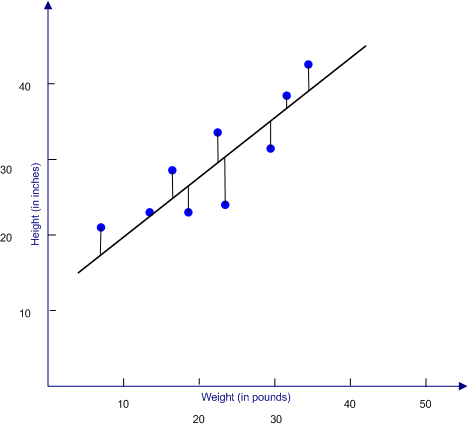
\includegraphics[height=0.6\textheight]{Assoc/residuos}
  \end{center}

  \begin{definition}
    Resíduos são a distância entre o dado observado e a reta estimada
    (modelo).
  \end{definition}
\end{frame}

\begin{frame}{Elementos da reta de regressão}
  \begin{itemize}
  \item Relembrando: a equação de uma reta é definida pela fórmula
    \begin{displaymath}
      \hat{y} = a x + b
    \end{displaymath}
  \item No caso da reta regressora:
    \begin{itemize}
    \item $y$ é a variável dependente
    \item $x$ é a variável independente
    \item $a$ é a inclinação
    \item $b$ é o intercepto
    \end{itemize}
  \item Assim, o objetivo da análise de regressão é encontrar os
    valores $a$ e $b$
  \end{itemize}
\end{frame}

\begin{frame}{Análise de Regressão}
  Para determinar a inclinação e o intercepto, usamos:
  \begin{itemize}
  \item as médias de $X$ e $Y$
  \item as variâncias de $X$ e $Y$
  \item o coeficiente de correlação $r$ entre $X$ e $Y$
  \item o tamanho da amostra $n$
  \item \ldots e algumas operações entre estes termos
  \end{itemize}
\end{frame}

\begin{frame}{Exercício}
  \begin{block}{Exercício}
    Dados de gastos com propaganda (x) e vendas (x), ambos em \$1000 de uma empresa.

\bigskip

\centering\begin{tabular}{|c|c|c|c|c|c|c|c|c|}
\hline
x & 2.4 &  1.6& 2.0 & 2.6 & 1.4& 1.6& 2.0& 2.2\\
\hline
y & 225& 184& 220& 240& 180& 184& 186& 215\\
\hline
    \end{tabular}

\bigskip

Qual é a {\em previsão} de retorno em vendas, para os seguintes gastos com propagandas?

\begin{enumerate}
\item 1.5
\item 1.8
\item 2.5
\end{enumerate}
  \end{block}

Fonte: Larson \& Farber.
\end{frame}

\begin{frame}{Exercício}
  \centering
  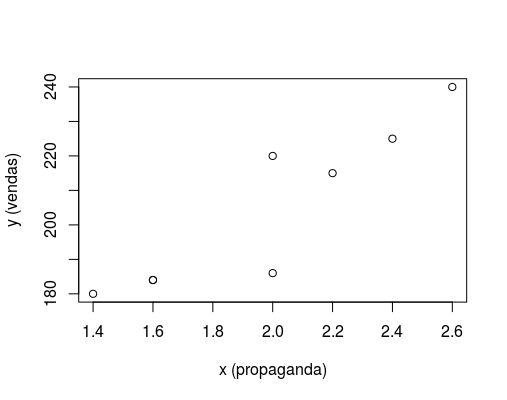
\includegraphics[width=\textwidth]{Assoc/regressao1}
\end{frame}

\begin{frame}{Exercício}
  \centering
  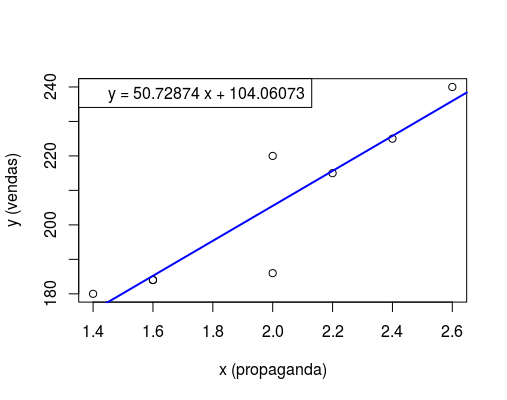
\includegraphics[width=\textwidth]{Assoc/regressao2}
\end{frame}

\begin{frame}{Exercício}
  \begin{block}{Cola}
        \begin{itemize}
        \item<1->  \alert{$y = 50.72874 x + 104.06073$}
        \item<1->  $x_1 = 1.5$
        \item<1->  $x_2 = 1.8$
        \item<1->  $x_3 = 2.5$
        \end{itemize}
  \end{block}
  \begin{block}{Solução}
    \begin{enumerate}
    \item $y_1 = 50.72874 x_1 + 104.06073 = 50.72874 \times \alert{1.5} + 104.06073 = 180.1538 \approx \alert{180.2}$
    \item $y_2 = 50.72874 x_2 + 104.06073 = 50.72874 \times \alert{1.8} + 104.06073 = 195.3725 \approx \alert{195.4}$
    \item $y_3 = 50.72874 x_3 + 104.06073 = 50.72874 \times \alert{2.5} + 104.06073 = 230.8826 \approx \alert{230.9}$
    \end{enumerate}
  \end{block}
\end{frame}

\begin{frame}{Análise de Regressão}
  \begin{center}
      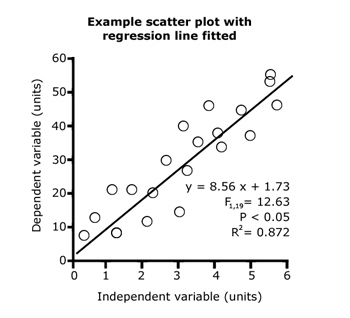
\includegraphics[height=0.6\textheight]{Assoc/residuos2}
  \end{center}

  \begin{itemize}
  \item A qualidade do ajuste do modelo de regressão é determinado
    pelo \alert{coeficiente de determinação} $r^2$
  % \item A semelhança de nomenclatura com o coeficiente $r$ não é mera
  %   coincidência.
  \end{itemize}
\end{frame}

  % Encontrando a inclinação e o intercepto da reta, podemos estimar
  % $\hat{Y}$ para valores arbitrários de $X$.

% \subsection{}

% \begin{frame}{}
%   \begin{itemize}
%   \item 
%   \end{itemize}
% \end{frame}

% \begin{frame}{}
%   \begin{itemize}
%   \item 
%   \end{itemize}
% \end{frame}

\subsection[$R^2$]{Coeficiente de Determinação $r^2$}

\begin{frame}{Coeficiente de Determinação $r^2$}
  \begin{definition}
    O \alert{coeficiente de determinação} $r^2$ é a relação da
    variação explicada com a variação total.
  \end{definition}
  \begin{displaymath}
    r^2 = \frac{\text{variação explicada}}{\text{variação total}}
  \end{displaymath}
  \begin{itemize}
  \item Lembrando: $r^2$ é o quadrado de $r$!
  % \item Este valor tem uma interpretação prática mais fácil, que
  %   veremos em breve
  \end{itemize}
\end{frame}

\begin{frame}{Coeficiente de Determinação $r^2$}
  \begin{itemize}
  % \item A variância dos dados pode ser explicada de várias formas
  \item Qual é a porcentagem da variação dos dados pode ser explicada
    pela reta regressora?
  \item O coeficiente $r^2$ é a fração da variância que é
    compartilhada entre $X$ e $Y$.
  \item Como $r$ está sempre entre -1 e 1, $r^2$ está sempre entre 0 e
    1.
  \end{itemize}
\end{frame}

\begin{frame}{Coeficiente de Determinação $r^2$}
  \begin{itemize}
  \item Além disso, $r^2 \le |r|$
  \item Por que?
  \end{itemize}
  \begin{block}{}
    Compare os seguintes números entre 0 e 1:
    \begin{displaymath}
      \frac{1}{2} \text{ e } \left(\frac{1}{2}\right)^2=\frac{1}{4} \Rightarrow
      \frac{1}{4} \le \frac{1}{2}
    \end{displaymath}
    \begin{displaymath}
      \frac{1}{3} \text{ e } \left(\frac{1}{3}\right)^2=\frac{1}{9} \Rightarrow
      \frac{1}{9} \le \frac{1}{3}
    \end{displaymath}
  \end{block}
\end{frame}


% \begin{frame}{Coeficiente de Determinação $r^2$}
%   \begin{itemize}
%   \item 
%   \end{itemize}
% \end{frame}


\section{Interpretação}
% \subsection{Interpretação}

\begin{frame}{Interpretação}
  \begin{itemize}
  \item Se a correlação é 0, então X e Y não variam juntos (independentes)
  \item Se a correlação é positiva, então quando uma aumenta, a outra
    aumenta em proporção direta (linear)
  \item Se a correlação é negativa, então quando uma aumenta, a outra
    diminui em proporção inversa (linear)
  \end{itemize}
\end{frame}


\begin{frame}{Cuidado!}
  \begin{itemize}
  \item Duas variáveis podem \alert{parecer} correlacionadas pois são
    influenciadas por uma terceira variável
  \item Ex: em alguns países a mortalidade infantil é negativamente
    correlacionada com o número de telefones per capita
  \item Mas comprar mais telefones não vai salvar crianças!
  \item Explicação alternativa: a melhoria da condições financeiras
    pode afetar ambas as variáveis
% tanto a quantidade de telefones, quanto a longevidade
    % infantil
  \end{itemize}
\end{frame}

\section{Causalidade}
% \subsection{Causalidade}


\begin{frame}{Causa x efeito}
  \begin{itemize}
  \item Se há uma relação de causalidade entre as duas variáveis, a
    correlação será não nula (positiva ou negativa)
  \item Quanto maior for a relação de dependência entre as variáveis,
    maior será o módulo da correlação.
  \item Se as variáveis não são relacionadas, a correlação será nula.
  \end{itemize}
\end{frame}

\begin{frame}{Causalidade?}
  \begin{itemize}
  \item Mas não podemos inverter a afirmativa lógica do slide
    anterior!
  \item Isto é, ao observar uma forte correlação, gostaríamos de
    concluir que uma variável \alert{causa} este efeito na outra
  \item Infelizmente isto não é possível!
  \item Lembre-se: a significância do teste indica a probabilidade de
    se cometer um erro do tipo I (falso positivo).
  \end{itemize}
  \begin{block}{Repita várias vezes mentalmente}
    Correlação não implica em causalidade.
  \end{block}
\end{frame}

% \begin{frame}{}
%   \begin{itemize}
%   \item 
%   \end{itemize}
% \end{frame}

\begin{frame}{Exemplo}
  Gasto com C\&T (EUA) x Suicídios por enforcamento
  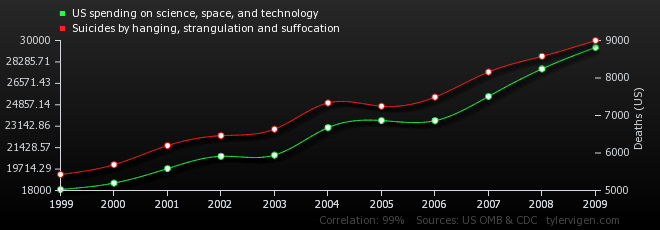
\includegraphics[width=\textwidth]{Assoc/us-spending-on-science-space-and-technology_suicides-by-hanging-strangulation-and-suffocation}

  Correlação: 0.992082

  (Fonte: Spurious correlations)
\end{frame}

\begin{frame}{Exemplo}
  Produção de mel x Prisões por posse de maconha
  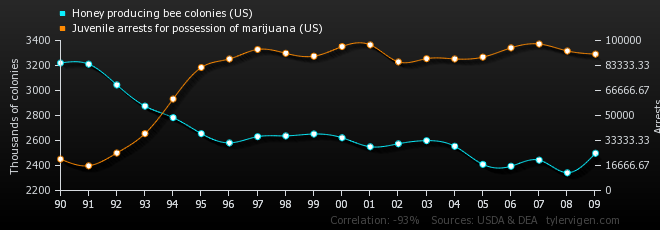
\includegraphics[width=\textwidth]{Assoc/honey-producing-bee-colonies-us_juvenile-arrests-for-possession-of-marijuana-us}

  Correlação: -0.933389

  (Fonte: Spurious correlations)
\end{frame}

\begin{frame}{Exemplo}
  Afogamentos em piscina x Filmes com Nicholas Cage
  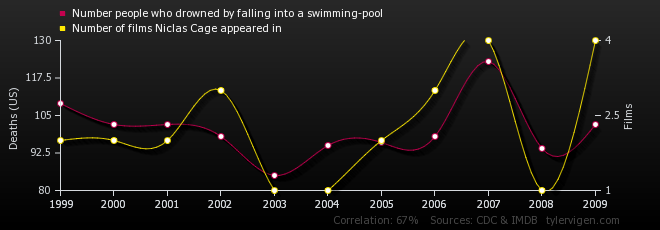
\includegraphics[width=\textwidth]{Assoc/number-people-who-drowned-by-falling-into-a-swimming-pool_number-of-films-niclas-cage-appeared-in}

  Correlação: 0.666004

  (Fonte: Spurious correlations)
\end{frame}

\begin{frame}{Causa e efeito}

  Ao encontrar uma forte correlação, deve-se sempre se perguntar:

  \begin{enumerate}
  \item Há uma relação direta de causa e efeito entre as variáveis? (X
    causa Y?)

  \item Há uma relação inversa de causa e efeito entre as variáveis?
    (Y causa X?)

  \item É possível que a relação entre as variáveis possa ser causada
    por uma terceira variável (ou mais) que não foi analisada?

  \item É possível que a relação entre duas variáveis seja uma
    coincidência?
  \end{enumerate}
\end{frame}

\section{Resumo}
\begin{frame}{Resumo}
  \begin{itemize}
  \item É necessário investigar a relação entre as variáveis!
  \item O que pode explicar a relação observada?
  \item Qual proporção (porcentagem) da variabilidade pode ser
    explicada pelas variáveis analisadas?
  \item Quão bem a reta regressora se ajusta aos dados?
  \end{itemize}
\end{frame}


% \begin{frame}{}
% \end{frame}

\end{document}
